\subsubsection{Sod Shock Tube}
\label{sec.tests.sodshock}

We begin the paper test suite with the classic one-dimensional Sod shock tube problem
\citep{Sod78}, which provides a good test of a hydrodynamical solver's
ability to resolve a clean Riemann problem with clear separation
between the three resultant waves.  These waves consist of a rarefaction fan, a
contact discontinuity, and a moderate shock.  The initial state is 
$\rho_{\rm L}, P_{\rm L} = 1.0, 1.0$ on the left of the boundary at 
$x=0.5$ and $\rho_{\rm R}, P_{\rm R} = 0.125, 0.1$ on the right.
All velocities are initially zero.  In
Figure~\ref{fig.sodshocktube}, we show the density solution at the
final time ($t=0.25$) for three of our hydro solvers -- the spatially third-order
PPM, as well as the two second-order \zeus\ and MUSCL schemes.  We use
100 cells across the domain, (which is a relatively standard choice in
code method papers) and show solutions both with and without adaptive
mesh refinement.  Without AMR (top row in Figure \ref{fig.sodshocktube}), it is
clear that the PPM scheme produces by far the cleanest solution with
all wave families crisply reproduced (in particular, the contact
discontinuity and shock).  \zeus\ and MUSCL produce similar results,
with MUSCL doing a slightly better job on the rarefaction fan.  In Figure
\ref{fig.sodshocktube}, we also show the integrated absolute deviation from 
the exact solution, $||E_1|| = \sum_i \Delta x_i |F(x_i)-{\rm Exact}(x_i)|$ 
, as well as the maximum deviation,
$||E_\infty|| = \mathrm{max_i}\left\{ \Delta x_i|F(x_i)-{\rm Exact}(x_i)| \right\}$.  
These numbers confirm the qualitative differences noted
previously.

We also run the same simulation but with two levels of AMR (using a
refinement factor of 2), triggered based on a normalized slope greater
than 10\% in the density.  This refinement criterion results in only
the refinement of strong gradients, and
does not include the rarefaction fan at late times.  The results are
shown in the bottom row of Figure~\ref{fig.sodshocktube}.  Using AMR,
the results are much better for all three methods, with much sharper
shocks and contact discontinuities and even a better representation of
the rarefaction wave, which is only refined beyond the root grid at
early times.  Although the results are improved for all methods, PPM
still produces the best result, as is shown clearly by the computed
error norms (displayed again in each of the individual panels).

\begin{figure}
\begin{center}
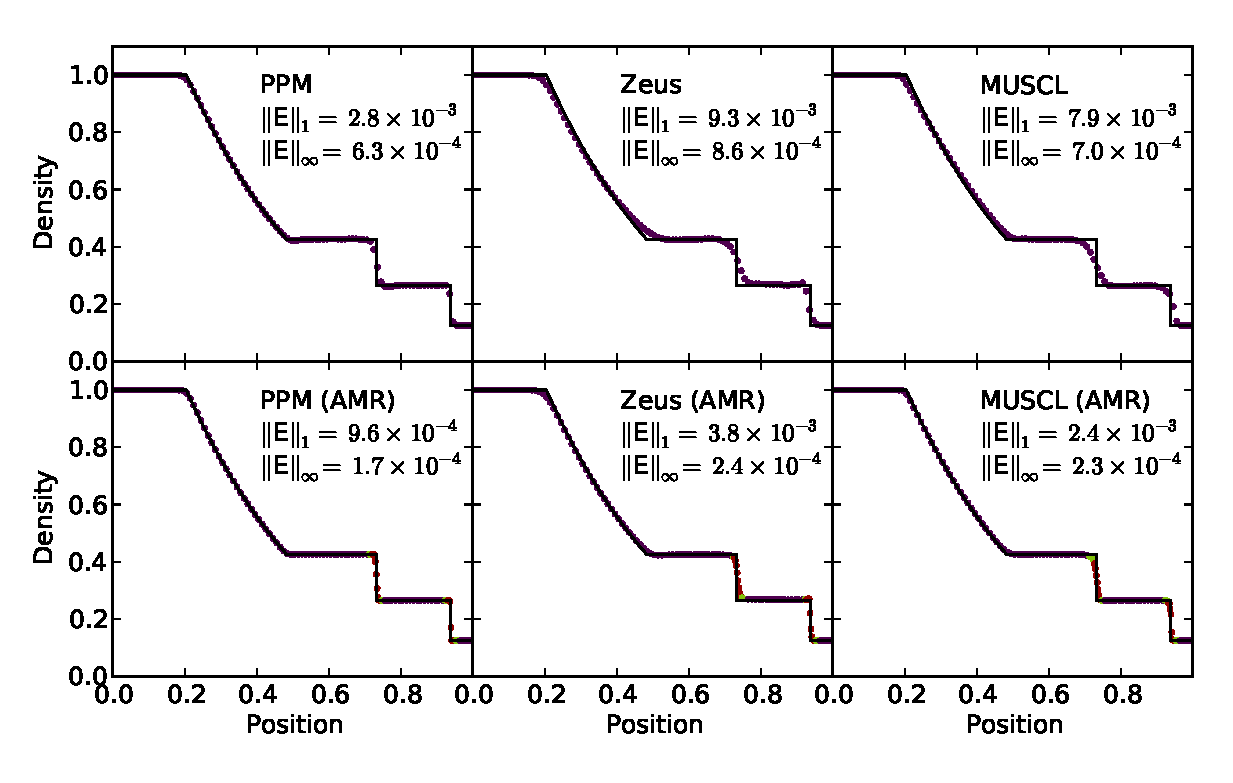
\includegraphics[width=\textwidth]{figures/SodShockTube.eps}
\caption{The density distribution of the classic Sod Shock Tube for
three different solvers (from left to right column) and with (bottom
row) and without (top row) AMR.  In each case 100 zones are used on
the root level and the results are shown at $t=0.25$.  All cells are
plotted and color-coded by level with purple 
indicating level 0, green level 1 and red level 2 (at the time shown, only small region
surrounding the contact discontinuity and the shock are refined).  In
each panel, we show the analytic solution as a solid line and the $E_1$
and $E_\infty$ error norms in the upper right.}
\label{fig.sodshocktube}
\end{center}
\end{figure}


